\chapter{Introducción específica}

En este capítulo se presenta un resumen de los conceptos más relevantes acerca de la red TCN y su implementación en las formaciones de Trenes Argentinos, y se detallan las diferentes tecnologías utilizadas para el desarrollo del dispositivo de captura.

\section{La red TCN}

La red TCN es una combinación jerárquica de dos buses de datos en los que se transmite información dentro de una formación ferroviaria. El Multifunction Vehicle Bus (MVB) interconecta los diferentes dispositivos presentes dentro de cada vehículo, y el Wire Train Bus (WTB) interconecta los diferentes vehículos. Los componentes de la red TCN están estandarizados en la norma IEC 61375-1. En la figura~\ref{fig:tcn-mvb-wtb} se muestra un diagrama simplificado de la arquitectura TCN.

\begin{figure}[htbp]
	\centering
    {
        \fontfamily{phv}
        \fontsize{9pt}{9pt}\selectfont
        \input{./Figures/tcn-mvb-wtb.pdf_tex}
    }
	\caption[Wire Train Bus y Multifunction Vehicle Bus]{Wire Train Bus y Multifunction Vehicle Bus.\footnotemark}
    \label{fig:tcn-mvb-wtb}
\end{figure}
\footnotetext{Dibujo del tren por Freepik\\(\url{https://www.freepik.com/free-vector/collection-different-types-trains_1114167.htm})}

Dado que el dispositivo desarrollado se conecta al bus MVB, a continuación se exponen las características principales de este bus de comunicación.

\subsection{El bus MVB}

El bus MVB interconecta diferentes dispositivos ubicados en el mismo vehículo o en diferentes vehículos que no son separados con frecuencia. El MVB puede direccionar hasta 4095 dispositivos, y proporciona tanto la interconexión de equipos programables entre sí como la interconexión de estos equipos con sus sensores y actuadores.

La estructura de MVB sigue el modelo OSI \cite{ISO7498-1}, en el que se definen siete capas de abstracción, cada una con una función específica para la transmisión de datos. A continuación se describen las capas de más abajo, que son las más relevantes para este trabajo.

La estructura de MVB sigue el modelo OSI \cite{ISO7498-1}, que establece siete capas de abstracción para la transmisión de datos. A continuación se describen las tres capas inferiores, que son las más relevantes para el desarrollo de este trabajo.

\subsection{Capa física}

El bus MVB ofrece tres opciones de medios físicos para la capa inferior:

\begin{itemize}
\item El medio Electrical Short Distance (ESD), para distancias de hasta 20~m, que soporta hasta 32 dispositivos por segmento, con transceptores de tipo RS-485.
\item El medio Electrical Middle Distance (EMD), para distancias de hasta 200~m, que soporta hasta  32 dispositivos por segmento, con transformadores y transceptores compatibles con la norma IEC 61158-2 \cite{iec61158_2}.
\item El medio Optical Glass Fibre (OGF), para distancias de hasta 2000~m, y soporta conexiones punto a punto o subredes de topología tipo estrella.
\end{itemize}

Puede haber diferentes buses en un vehículo, interconectados mediante un \textit{gateway} al bus WTB.
También es posible que el bus MVB abarque más de un vehículo, y en este caso la norma recomienda el medio EMD.
Un ejemplo de esta configuración se ilustra en la figura~\ref{fig:emd-esd-wtb}.

\begin{figure}[htbp]
	\centering
    {
        \fontfamily{phv}
        \fontsize{9pt}{9pt}\selectfont
        \input{./Figures/medios.pdf_tex}
    }
	\caption[MVB abarcando tres vehículos]{MVB abarcando tres vehículos.}
    \label{fig:emd-esd-wtb}
\end{figure}

En la figura~\ref{fig:segmento} se ilustra un segmento EMD.
Cada dispositivo conectado a un segmento EMD tiene dos conectores D-sub de 9 pines (DE-9) que van, respectivamente, al dispositivo anterior y siguiente en el segmento. Los dispositivos en los extremos del segmento tienen un terminador.

\begin{figure}[htbp]
	\centering
    {
        \fontfamily{phv}
        \fontsize{9pt}{9pt}\selectfont
        \input{./Figures/segmento-emd.pdf_tex}
    }
	\caption[Un segmento EMD]{Un segmento EMD.}
    \label{fig:segmento}
\end{figure}

En la figura~\ref{fig:db9} se muestra la configuración de pines de los conectores.
La transmisión de la señal digital se realiza mediante la tensión diferencial entre los pares Data\_N y Data\_P. La norma permite que haya una única línea (A) o dos líneas (A y B) para proporcionar redundancia.

\begin{figure}[htbp]
	\centering
    {
        \fontfamily{phv}
        \fontsize{9pt}{9pt}\selectfont
        \input{./Figures/db9-emd.pdf_tex}
    }
	\caption[Configuración de pines del conector D-sub de 9 pines del medio EMD]{Configuración de pines del conector DE-9 del medio EMD. Se omite por simplicidad la interconexión de los pines 6 a 9, que se utilizan para los terminadores.}
    \label{fig:db9}
\end{figure}

\subsection{Tramas}

Se denomina \textit{trama} a un paquete de datos transmitido por un dispositivo.
En el bus MVB se transmiten dos tipos de tramas:

\begin{itemize}
\item La trama \textit{master}, que es transmitida únicamente por el dispositivo maestro del bus.
\item La trama \textit{slave}, que es transmitida por un dispositivo esclavo en respuesta a una trama \textit{master}.
\end{itemize}

Todos los medios MVB operan a una velocidad unificada de 1,5~Mbit/s.
La información se transmite utilizando una codificación Manchester, que combina en una única señal la información y el \textit{clock}.

La transmisión de una trama se compone de un delimitador inicial (SD) de 9 bits de duración, los datos de la trama, una secuencia de verificación (CS) de 8 bits y un delimitador final (ED) de 2 bits de duración.
En los datos de la trama y la secuencia de verificación, un ``1'' se transmite como una transición negativa en el medio de una celda de bit, y un ``0'' se transmite como una transición positiva.
Los delimitadores de inicio para las tramas \textit{master} y \textit{slave} son diferentes, y se denominan MSD y SSD.
En la figura~\ref{fig:manchester} se muestra a modo de ejemplo la transmisión de una trama \textit{master} en el medio EMD.

\begin{figure}[htbp]
	\centering
    {
        \fontfamily{phv}
        \fontsize{9pt}{9pt}\selectfont
        \input{./Figures/manchester.pdf_tex}
    }
	\caption[Transmisión de una trama master]{Transmisión de una trama \textit{master}.}
    \label{fig:manchester}
\end{figure}


\subsection{Telegramas}

Una secuencia de una trama \textit{master} seguida de una trama \textit{slave} conforman un \textit{telegrama}, como se muestra en la figura~\ref{fig:telegrama}.

\begin{figure}[htbp]
	\centering
	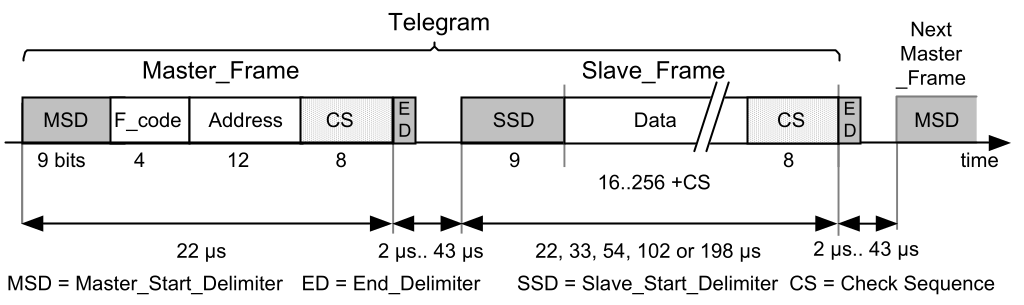
\includegraphics[width=1\textwidth]{./Figures/telegrama.png}
	\caption[Un telegrama MVB]{Un telegrama MVB.
        \\ \todo{CAMBIAR: La imagen original tiene copyright.}}
    \label{fig:telegrama}
\end{figure}

Las tramas \textit{master} tienen una longitud fija de 16 bits (sin contar los delimitadores), e incluyen:

\begin{itemize}
\item Un código de 4 bits llamado \texttt{F\_code}, que indica el tipo y tamaño de la trama \textit{slave} esperada a continuación.
\item Un campo de 12 bits, que puede contener una dirección de destino, o parámetros específicos al \texttt{F\_code}.
\end{itemize}

Todos los dispositivos conectados al bus decodifican la trama \textit{master}. El dispositivo encuestado luego responde con su trama \textit{slave}, que a su vez puede ser recibida por otros dispositivos.

Son de particular interés los telegramas con \texttt{F\_code} entre 0 y 4. Este tipo de telegramas son denominados \texttt{Process\_Data}, y en este caso el campo de 12 bits contiene una dirección lógica que se interpreta como un \textit{puerto}. Cada puerto está asociado unívocamente a una \textit{variable}, que puede contener uno o más valores como la velocidad actual, la tensión de red, el estado de las puertas, etc. Cada dispositivo \textit{slave} almacena uno o más puertos, y al ser encuestado responde con el valor actual de la variable correspondiente.

\section{TCN en las formaciones de Trenes Argentinos}

En la figura~\ref{fig:tms} se muestra un diagrama de la topología de la red TCN en un segmento de una formación, compuesto por 3 vehículos EMU. Los buses MVB están implementado con el medio físico EMD.

\begin{figure}[htbp]
	\centering
	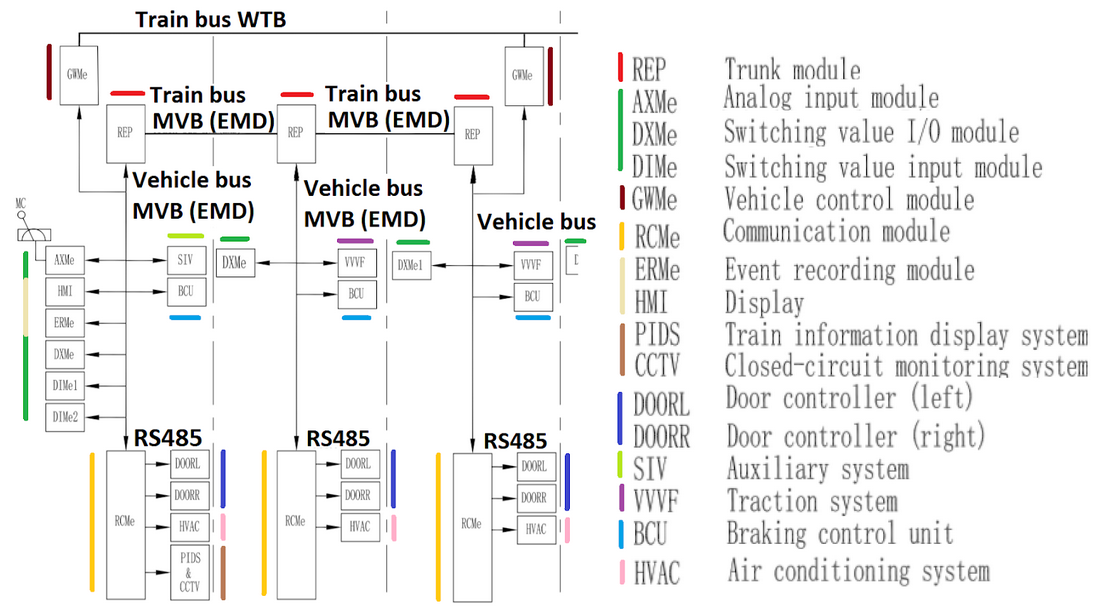
\includegraphics[width=1\textwidth]{./Figures/tms.png}
	\caption[Topología de la red TCN en una formación de Trenes Argentinos]{Topología de la red TCN en una formación de Trenes Argentinos.
        \\ \todo{REVISAR: Rehacer para mejorar la legibilidad.}}
    \label{fig:tms}
\end{figure}

En la figura~\ref{fig:rcme} se muestra una fotografía del interior de un \textit{rack}, en la cabina del conductor de una formación de la línea Mitre. En la imagen se observa uno de los módulos conectados en el bus MVB, el módulo de comunicación RCMe, que controla las puertas (DOORR, DOORL), el sistema de aire acondicionado (HVAC) y el sistema de información al pasajero (PIDS). En el panel frontal del módulo RCMe, los conectores DE-9 X1 y X2 corresponden al bus MVB.

\begin{figure}[htbp]
	\centering
	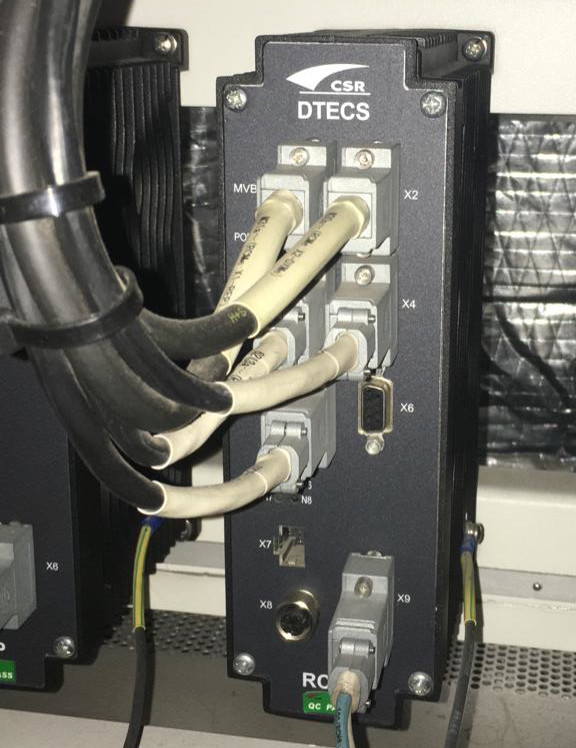
\includegraphics[width=0.5\textwidth]{./Figures/RCMe.jpeg}
	\caption[El módulo de comunicación RCMe]{El módulo de comunicación RCMe presente en un EMU.
        \\ \todo{REVISAR: Agregar indicaciones y una leyenda para cada conector.}}
    \label{fig:rcme}
\end{figure}

En la cabina del conductor, la pantalla HMI (Human Machine Interface) tiene un modo de operación que permite visualizar el valor de algunas variables que son transmitidas periódicamente en forma de \texttt{Process\_Data}. En la figura~\ref{fig:hmi} se puede ver que en el puerto 0 hay una variable de 16 bits cuyo valor binario actual es 1100 0001 0110 0101, o 33702 si se interpreta como un número decimal.

\begin{figure}[htbp]
	\centering
	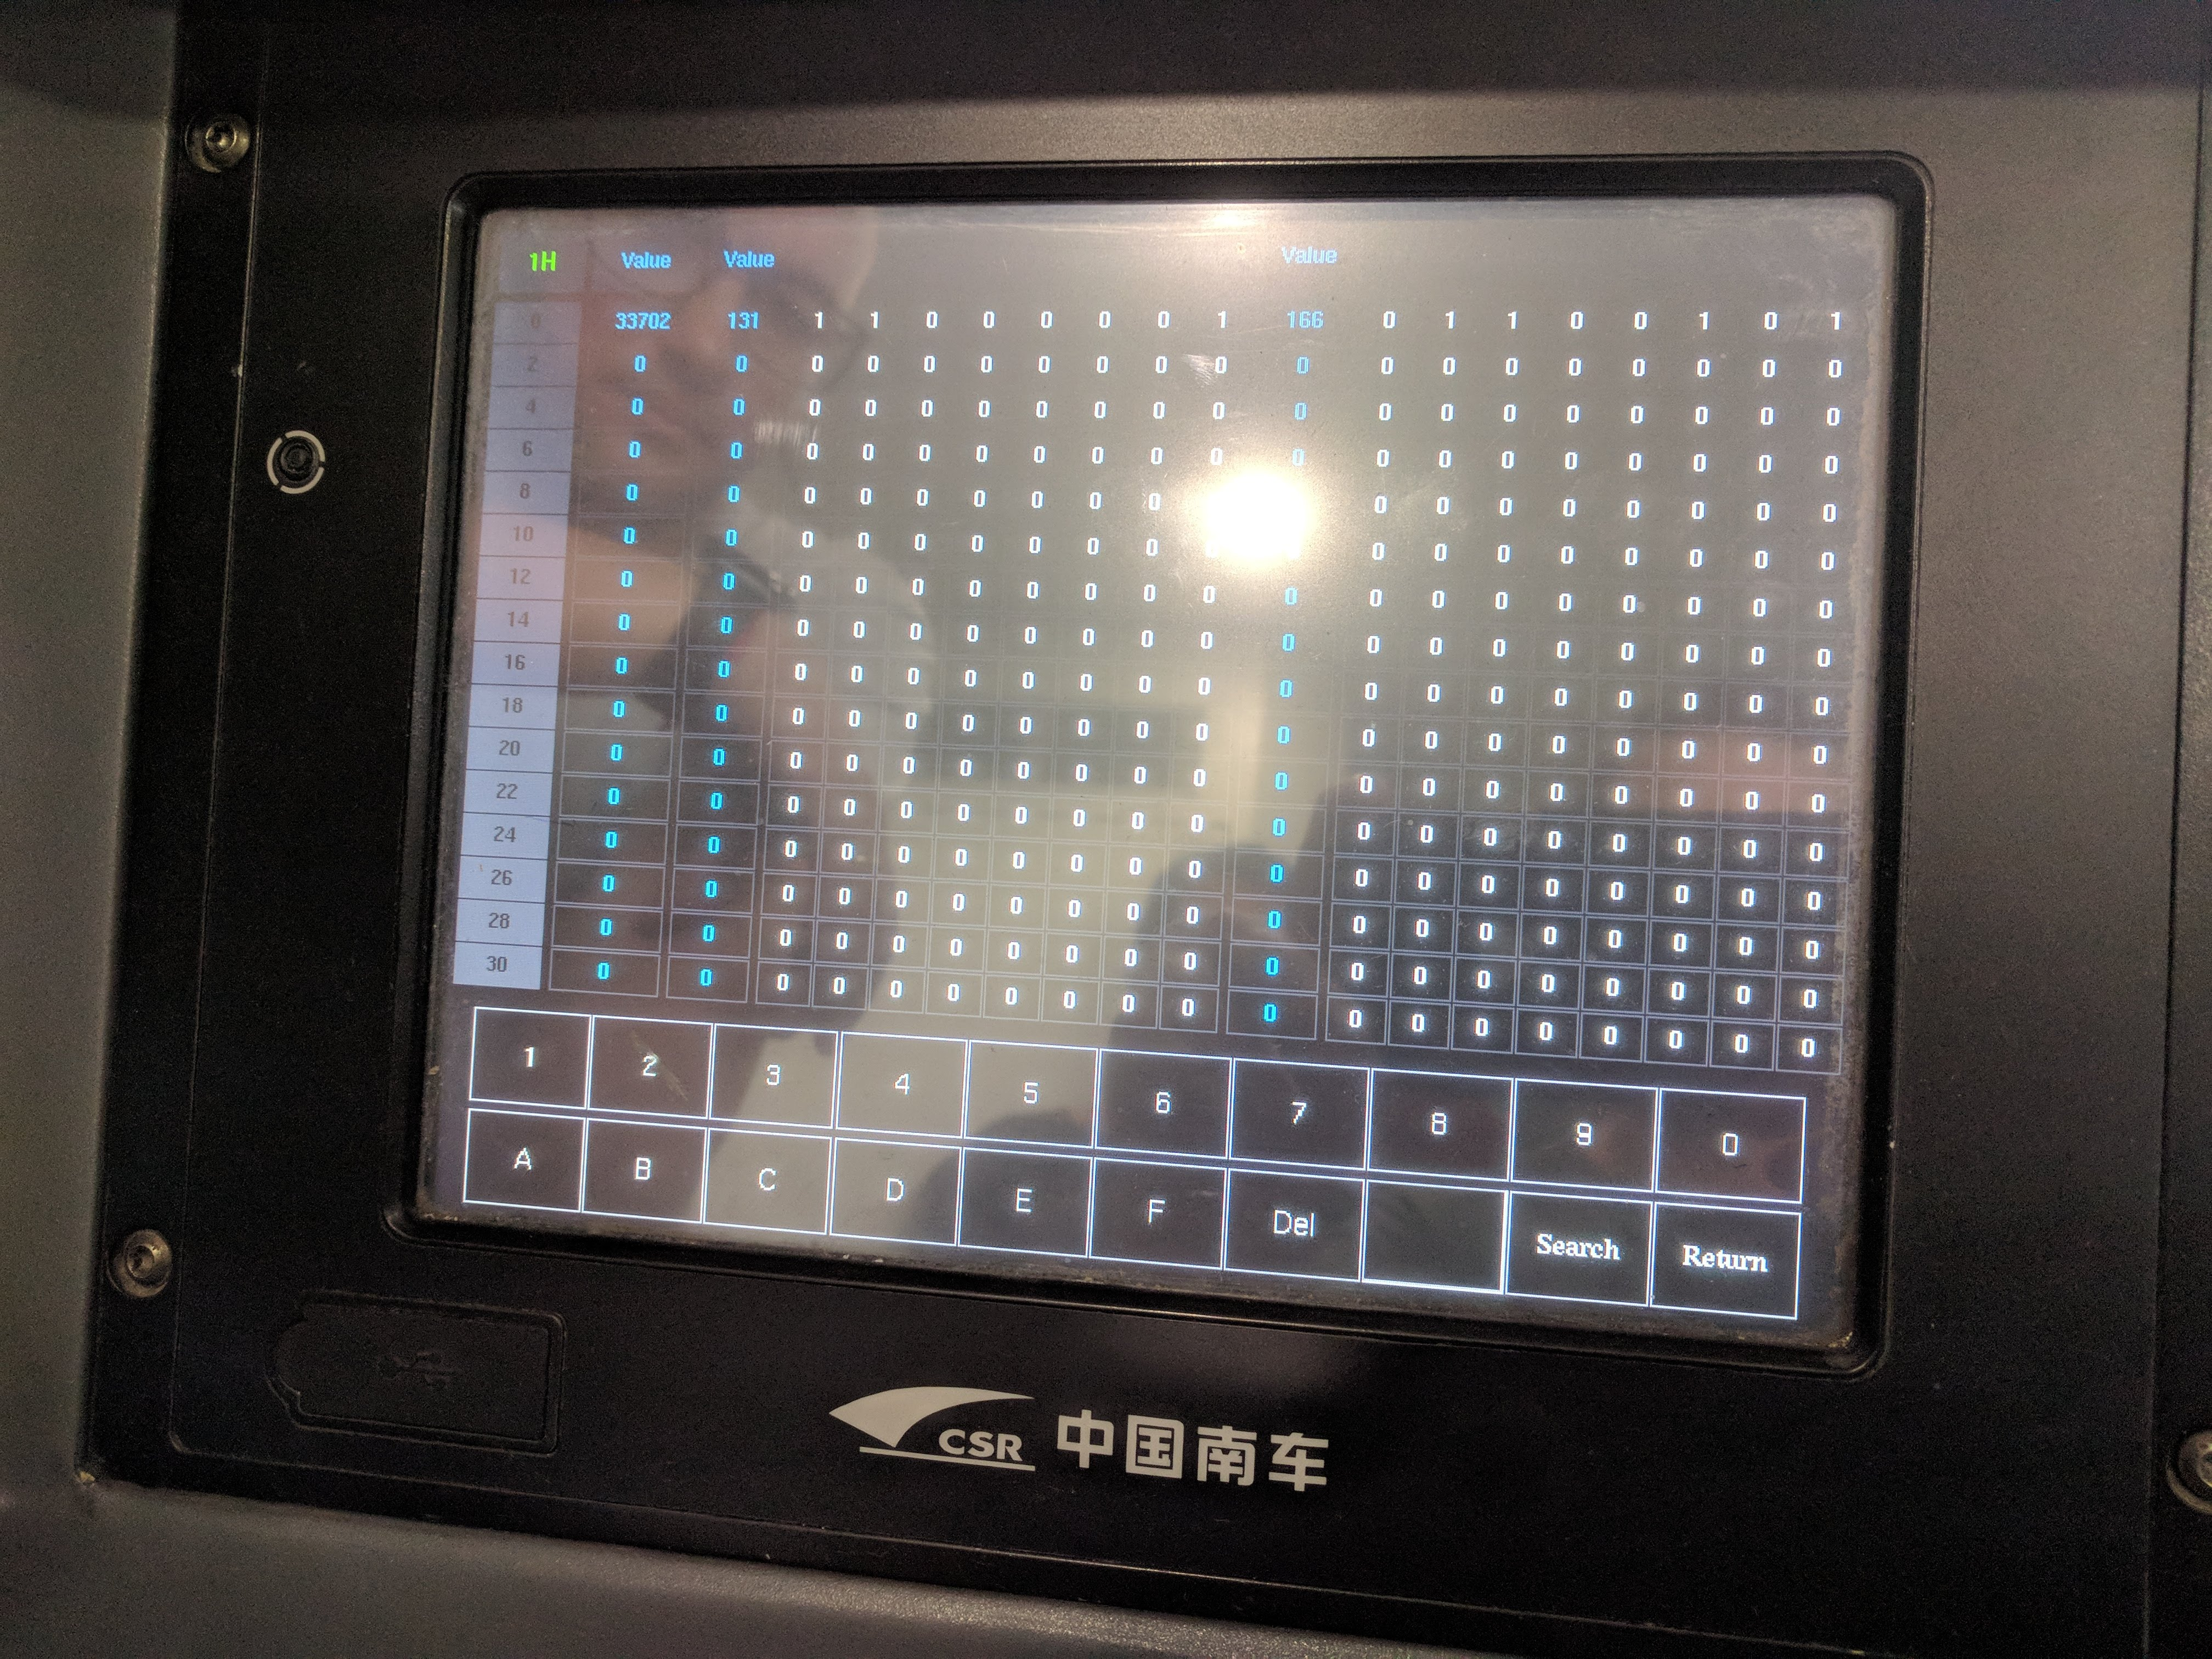
\includegraphics[width=1\textwidth]{./Figures/hmi.jpg}
	\caption[El HMI mostrando algunas variables]{El HMI mostrando algunas variables.}
    \label{fig:hmi}
\end{figure}



\section{Componentes del sistema}
